\chapter{Seizure Prediction}

Electroencephalograms(EEGs) capture the electromagnetic 
potential of aligned neurons firing in unison. 
Although a number of correlations between 
EEG and physiological phenomena have been found the relation between EEG and the dynamics of local neural circuitry are not well-understood \cite{eeg}. 
One difficulty is relating in vitro behavior of individual neural cells or small clusters of cells with the more complex 
large scale variations recorded by the EEG signal.  
In the case of the epileptic neuropathology, 
the challenge is to relate better known 
local cellular mechanisms to 
the spread synchronized neuronal firing associated with 
epileptic seizures. Making this connection between 
the larger scale electromagnetic phenomena recorded 
by the EEG signal and local neural dynamics is 
not the goal of this Chapter. Instead, this was 
a preliminary study to determine whether 
a seizure response to a locally applied stimulus
could be predicted based EEG recorded prior to the stimulus.
An additional aim of this chapter is to compare 
classification models based on the segmentation of 
EEG features based on the $\varepsilon$-complexity
coefficients.

% The results, on the other hand, were intended to 
% inform additional studies of the dynamics 
Using a 4 minute window of EEG taken from an 
epilepsy prone mouse we predict whether a stimulus
will induce a seizure response.  
A small set of spectral and non-linear 
features are calculated on six EEG channels. 
Change points in the $\varepsilon-$complexity coefficients
are used to segment the features and the results 
are compared to other segmentation methods.
We also compare the features and 
channels predictive of seizure outcomes with 
the variation in feature distributions of trials with
seizure and non-seizure outcomes. Because predictions are 
made on a channel-by-channel basis, we also able to compare 
how features predictive of seizure outcomes vary 
by channel and brain region.


\section{Introduction}

EEG are non-stationary signals 
marked by transient waveforms and 
apparent regime changes over relatively short periods of times.
A common method of analyzing EEG is to compute 
some set of features on the raw signal EEG signal
and use these features as input to one or more classifiers. 
These features often combine a decomposition 
of the signal, for example, spectral, wavelet, principal component(PCA) or independent component(ICA) decompositions, with 
some linear or non-linear features\cite{alotaiby2014}.
Signal decomposition and feature selection
serve to reduce the high-dimensional 
EEG signal to a more interpretable feature set by 
averaging feature values over a sliding window.
One drawback of this method is that the process of averaging over arbitrary windows may obscure important 
features associated with the varying dynamics of the brain. 


Here, we use a set of spectral features and 
non-linear features to predict seizure outcomes. 
However, instead of segmenting the signal on uniform partitions
the segmentation is based on changes in the $\varepsilon-$complexity coefficients.
The $\varepsilon-$complexity coefficients were designed to 
capture discontinuities or regime changes in a signal. By 
partitioning the feature space at changes in the 
complexity coefficients we hope to capture features are 
more homogeneous segments. 

We compare classification performance based on 
several segmentation schemes, using both the complexity coefficients 
and a set of uniform break points to partition the features.
For each of these models, the prediction of seizure outcomes 
is based on features computed on single EEG channels.
Feature extraction and classification based on individual channels allows us to make more fine-grained inferences about the combination of feature and region that are associated with a seizure response.

% The $\varepsilon-$complexity feature was develope with 

% The iEEG -- which I will refer to simply as EEG --
% signal captures changes in field potential caused by large 
% groups of aligned neurons firing synchronously. The LFP sensors
% capture a signal from a smaller cluster of neurons.

% a way to detect changes in the underlying dynamics that generate some signal. Specifically, the analysis of EEG was a motivating test case. EEG signals measure changes in 
% electrical potential generally at the outer layer or cortex of the brain. 

% \section{Seizure Prediction}


\section{EEG Data}

The EEG data were gathered from 4 mice with a genetic 
mutation in the voltage-gated sodium channel gene Scn1a. 
A similar mutation is responsible for the Dravet syndrome 
and the mutation results in early onset epileptic seizures \cite{ito2013}.
The mice were equipped with 4 intracranial(iEEG) electrodes ---intracranial sensors placed directly on the brain cortex ---  
along with 2 local field potential (LFP) electrodes located 
 in the thalamus. The mice were genetically modified to produce a 
 light sensitive protein, an opsin. This allows for direct 
 stimulation of neurons with a laser pulse train. The stimulus is designed to induce a seizure in the mouse.
 
% \begin{figure}[!htbp]
%   \begin{center}
%   % \begin{picture}(60,60)
%   % ./figs/coeff-interp-simple-functions1.pdf
%   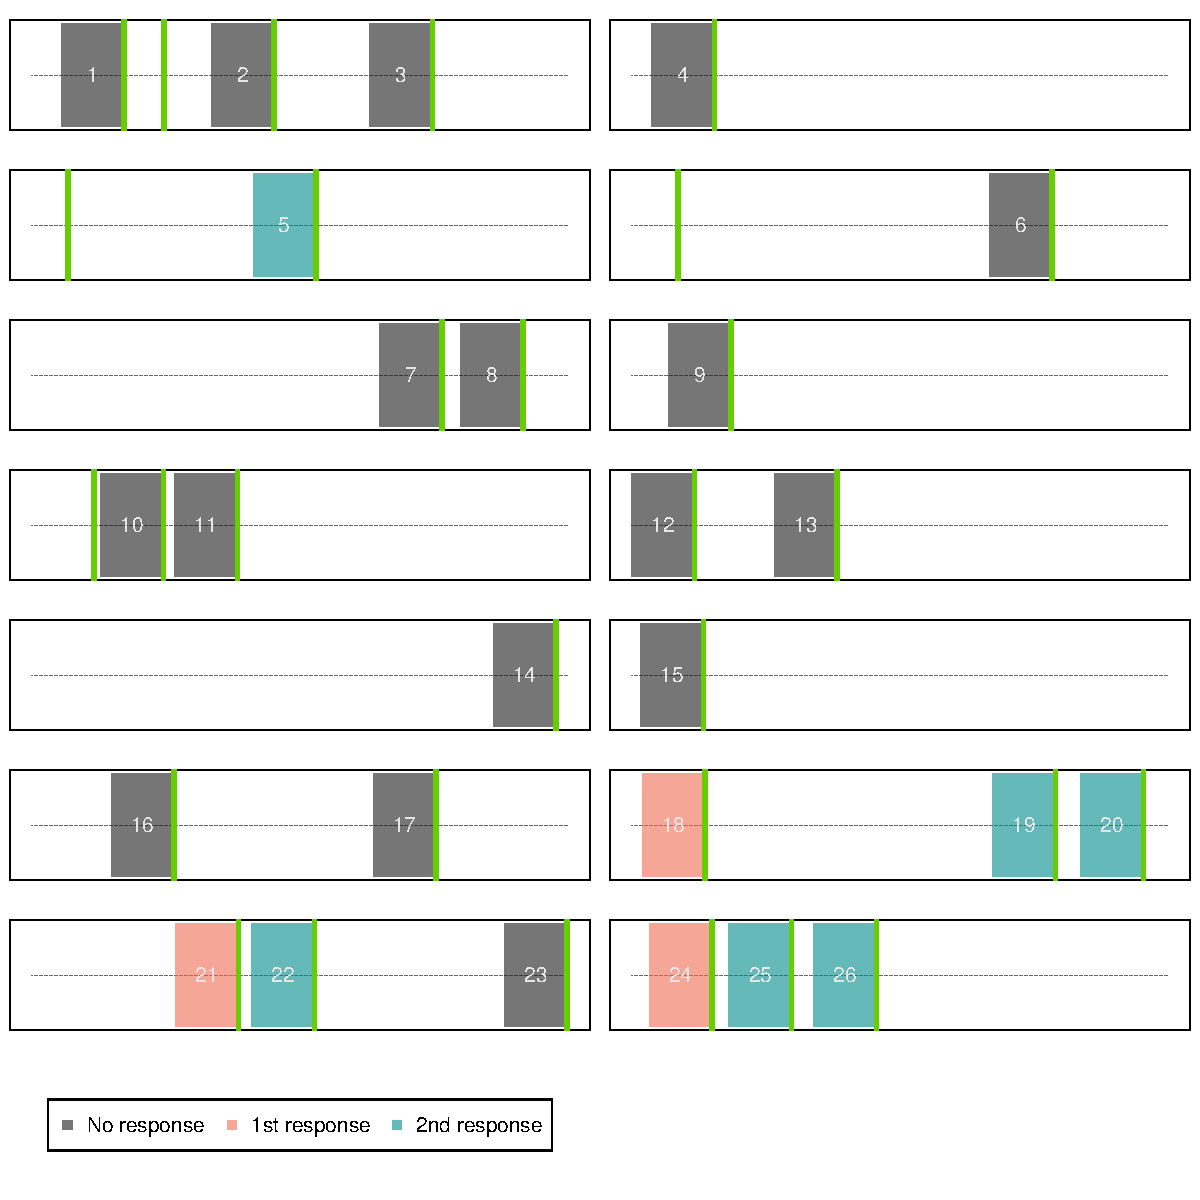
\includegraphics[width = \textwidth, keepaspectratio]{./figs/trialplot.pdf}
%   % \end{picture}
%   \end{center}
%   \label{fig:trialplot} 
%   \caption{Schematic plot of trial data. Each rectangle 
%            represents a single time period. The green 
%            vertical bars indicate applications of the stimulus.}
% \end{figure}

Data was gathered from 13 distinct time periods during which the 
stimulus was applied between one to four times. There were 26 trials in total. 
The 4-minute segments preceding the stimulus was used 
to predict outcomes.
 The result of each trial was were coded as either a seizure 
 or no seizure and we refer to a seizure as a positive response. 
Coding was based on the visible response of the 
mouse. The EEG signals around the stimulus period were also visually examined to check the accuracy of the coding.
The iEEG and LFP signals was sampled at 1220.7 Hz and
a bandpass filter removed frequencies below 0.5 Hz and greater
than 300 Hz. A notch filter was applied at 60 Hz and its harmonic frequencies. 


\section{EEG Features}

The features consisted of windowed spectral band power
estimates, variance and two non-linear features.
The power in frequency bands 
delta, theta, alpha, beta, and gamma was calculated 
as the integral of the spectral density $f(\lambda)$ 
computed as a smoothed periodogram. For example, 
delta band power, $\delta B$, corresponds to 
the frequency band $0.5-4Hz$ and integrates  
$f(\lambda)$ over over this interval
\[
  \delta B = \int_{0.5}^{4} f(\lambda) d\lambda. 
\]
The frequency bins corresponding to the remaining
the theta, alpha, beta and gamma frequency bands are 
$ 4-8Hz, 8-12Hz, 12-30Hz, 30-100Hz$. Relative 
band power, band power divided by total power, 
was used as the final feature.

A smaller set of non-linear features was chosen 
based on their ability to 
classify the simulation groups used in Chapter 3. 
Features that did not increase the performance of a random 
forest classifier were omitted from the final feature set.
The initial set of features were sample entropy,
and permutation entropy, spectral entropy, a Hurst 
parameter estimator, wavelet variance, a fractal dimension estimator and signal variance. Of these, variance, spectral entropy and the Hurst parameter were used in our final classifier.

%  were tested for their ability to discriminate between the same two groups of simulations used in Chapter 3 to test the approximation methods used in estimating complexity coefficients. Based on these results, spectral entropy, fractal dimension, the Hurst parameter and the wavelet coefficients, along with the spectral band power features and the complexity coefficients were computed on the EEG. In informal testing
% with a baseline classification model, the wavelet coefficients did not improve classification results and were removed from the final feature set. Given more data, feature selection might have been better performed through cross-validation on a training set. On the other hand, one of our goals was to work with a reduced feature set that was more readily interpretable. 


 \textit{Spectral entropy} is a measure of the distribution of 
 power in the spectrum of a signal. 
\[  
  SE = - \int_{-\pi}^{\pi} f_x(\lambda) \log f(\lambda) d \lambda.
\]
We have defined the Hurst parameter, a measure of long-range 
dependence, in Chapter 2. The Hurst parameter was estimated using the corrected empirical Hurst exponent\cite{weron2002}.  


All features were calculated on non-overlapping 2 second intervals. The final list of feature used in classification was 
\begin{enumerate}
\item Delta, theta, alpha, beta, gamma 
\item Spectral entropy 
\item Hurst parameter
\item Variance
\end{enumerate}

The complexity coefficients were used to segment the features
but were not included as features in the final set of 
classifiers.
All features were computed on 2 second non-overlapping windows.
% The variogram estimator of fractal dimension, $\hat D$ was also computed but was omitted from the final models as the feature appeared closely correlated with the complexity coefficient $B$. 


\section{Classification Procedure}

The classification procedure takes place in four main 
steps.
For each channel, the features are computed on 2 second 
intervals. The resulting set of features is segmented based on changes in the complexity coefficients. 
The weighted averages of the features on these segments is
then used as training set for the classifier. Classifier
performance was evaluated using 5-fold cross-validation
and positive responses were even spread across the 
5 test sets.


% We selected a small set of features for our classifier. 
% These included the band power of the  
% frequency bands delta, theta, alpha, beta and. 
% Spectral features need 
% to be computed over a windowed section of the time series 
% that is some multiple of the lowest frequency being computed 
% in order for the power estimates to have some statistical 
% validity. So using spectral features inherently reduces 
% the dimensionality of the data, for example, from several 
% thousand points a set of six values representing the 
% band power of some window of frequencies will be computed. 
%  Features including the 
% complexity coefficients are computed on 2 second intervals. 
% Change-points in the complexity coefficients are then 
% used to segment the features. The final predictor 
% is the mean of the features computed on each segment.
% The basic steps used are outlined below.

 %   \begin{algorithm}[!htbp]
 %    \label{alg:segmenet}
 %  \caption{Single channel segment classifier \label{alg:ecomplex}}
 %  \DontPrintSemicolon
 %  \SetAlgoLined
 %  \SetKwInOut{Input}{Input}\SetKwInOut{Output}{Output}
 %  \Input{$ \mathcal{F} $ a set of multivariate time series
 %      $\textbf{f} $ corresponding of length $N$.}
 %  \Input{$\mathcal{L}_f$ a set of labels $l_f$ for each time series 
 %  $ \textbf{f} $ }
 %  \Input{$\mathcal{X}$ a set of time series $x_f$ of length $N$ 
 %  used to partition each $\textbf{f}$.} 
 %  \Output{$\mathcal{M}$ a trained classification model.}
 %  % \tcp{initialize array}
 %   % Initialize the array epsilons $\leftarrow [0]$   \;
 %  \BlankLine 
 % \ForEach{$f$ in $\mathcal {F}$} {    
 %    % \tcp{initialize array}    
 %   Compute the change points for $\mathcal{x}_f$
 %      $p_f \leftarrow$  change_pts($\mathcal{X}_f$)
 %   Segment $f$ on change points $x_f$
 %     $\{ f \} \leftarrow f$
 %    \ForEach{$f$ in $\mathcal{F}$} {
 %      % \tcp{Compute the approximation error}
 %        Compute the approximation error \\ 
 %        $\varepsilon_{h,f} \leftarrow 
 %       \frac{1}{N}\norm{f_h - X_{h} }^2$.  \;
 %      % mse\leftarrow \varepsilon_{h,f}$
 %    } 
 %     Find minimium error over all $f$  \\
 %     epsilons$_h$ $\leftarrow \min \varepsilon_{h,f}$. \;
 %  }
 %  Fit a least squares linear model \\
 %   $A,B$ $\leftarrow$ lm(epsilons$_h$ $ \sim \{ \mathbb{S}_h \} $.) \;
 %  \end{algorithm}

\begin{enumerate}
  \item For each channel compute set of features
        on regular intervals including 
        $\varepsilon-$complexity.
  \item For each channel, compute the change points 
        in $\varepsilon-$complexity. 
  \item For each trial, segment all features using the change point 
        set computed in the previous step. 
  \item Compute the mean of each feature on the 
        segments. 
   \item Label the means of the segments 
         in a training 
         set with the label of the full time 
         series and use this set to train 
         a classifier.
   \item Train a classifier on the means of the 
         segments. 
  \item  Using the held-out test set, 
         compute the class probability of each 
       segment of the test trial using the trained 
         classifier. 
  \item  For each trial the sum of the prediction probabilities of each segment, weighted by segment length, determine the final class probability.
\end{enumerate} \label{alg:segment-alg}

In the case of a uniform partition of the features, this
the method is equivalent to simply using the average class probability for each segment to classify the trial.

% \subsection{Random Forest Classifier}

In theory, any classifier, or several classifiers could be used in steps 5 and 6. We used a random forest classifier. The random forest is constructed from a large number of individual decision trees. For numeric data, the decision trees partition the feature space into $d-$dimensional rectangles each labeled with a class\cite{friedman2001}. The decision trees branches correspond to partitions of the feature space. For each branch, a subset of the features are chosen and the split is made in order to increase the class purity of each partition. The final prediction is based on the combined vote of the individual trees.  In addition to random selection of features, a random subset of observations are used to build each tree. This allows for an out-of-bag(OOB) estimate of the classifier 
accuracy which is calculated by classifying each observations using the set of trees which were built without seeing that observation \cite{breiman2001}.

The effect of individual features on the classification outcomes
can be less transparent for non-linear classifiers like random forest
when compared to regression-based classifiers. However, the 
importance of the variable in discriminating classes can 
be recovered from the classification trees. 
We report the mean variable importance of the random forest classifiers determined by the mean decrease in the 
Gini index across all branches
\cite{breiman2001}. The Gini index measures node purity, or 
the homogeneity of a class in a given node resulting from 
some division of the feature space. Informally, for binary 
classification variable importance measures how well a feature divides two classes into homogeneous cells.
\begin{figure}[!htbp]
  \begin{center}
  % \begin{picture}(60,60)
  % ./figs/coeff-interp-simple-functions1.pdf
  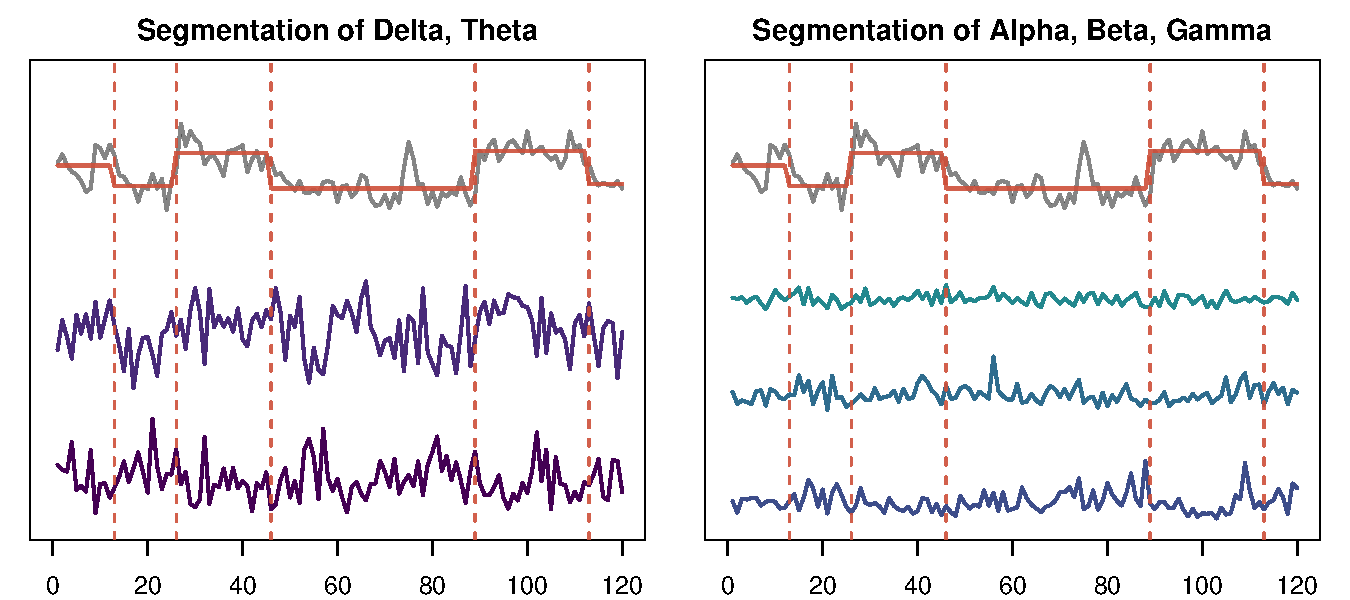
\includegraphics[width = \textwidth, keepaspectratio]{./figs/eeg-segment-plot.pdf}
  % \end{picture}
  \end{center}
  \label{fig:segplot} 
  \caption{Spectral features segmented on changes in the B complexity coefficient.}
\end{figure}

\section{Model Performance}

We begin by defining several terms we will be using to describe classifier performance. We term a seizure a 
positive response or simply a response. A  
\textit{true positive}  
is an accurate prediction of a seizure while a 
 \textit{true negative} is an accurate prediction of a non-response. 
The  \textit{sensitivity} of the classifier is then 
defined as the proportion of true positives to total 
positives
\[
  \frac{\text{True positives}}{\text{Total Positives}}
\]
 and  \textit{specificity} is the total of true 
negatives to total negatives:
\[
  \frac{\text{True Negatives}}{\text{Total Negatives}}.
\] 
We use the term accuracy to refer to balanced accuracy
\[
  \text{Balanced Accuracy} = \frac{\text{Sensitivity + Specificity}}{2}.
\] 
We also report AUC, or area under the ROC curve: see 
Figure \ref{fig:eegroc} for an example ROC curve from two 
of the classifiers tested. The 'curve' is the plot 
of the sensitivity against the false positive rate or 
$1 - $specificity and a higher AUC corresponds to a better performing classifier. An AUC of 1 indicates the correct classification of 
all observations.

A baseline classification model was built using the mean of each of the 8 features on the six channel resulting in 48 features. A random forest classifier was trained on these features and the out-of-bag classification results are reported in table \ref{tab:baseline}.
This baseline model classifies the over represented class, 
the negative or no-seizure responses, with 93\% accuracy but 
classification of a seizure response was no better than random.
% Asymptotically this is an unbiased estimate the error on a

 \begin{table}[!htbp] \centering 
 
\begin{tabular}{@{\extracolsep{5pt}} cccc} 
\\[-1.8ex]\hline 
\hline \\[-1.8ex] 
 & Sensitivity & Specificity & Accuracy \\ 
\hline \\[-1.8ex] 
1 & $0.544$ & $0.935$ & $0.740$ \\ 
\hline \\[-1.8ex] 
\end{tabular} 
 \caption{Classification performance of baseline classifier.} 
  \label{tab:baseline} 
\end{table} 


% \begin{table}[!htbp]
% \begin{center}
%   \begin{tabular}{ | c | c |  c|} 
%   \hline 
%  Sensitivity & Specificity  &  Accuracy  \\ \hhline{|=|=|=|}
%   0.54  &  0.94     &    0.74  \\ \hline
% \end{tabular}  
% \caption{Prediction performance for baseline classifier.}
% \label{tab:baseline}
% \end{center}
% \end{table}

We compared six models to this baseline model. For each 
model a different partition scheme was used. For the models
using complexity coefficients we label the models $A, B, A+B$,
 where the label corresponds to the complexity coefficient 
 or coefficients whose change points determined the
 partition. For example, the $A + B$ model partitions
 features based on the union 
of the change points of both complexity coefficients $A$ and 
$B$. 
For three other models we partitioned features into regular 
segments of length $8, 15$ or $30$. We refer to these models
by the number of partitions.

The performance of these models was assessed using 
5-fold cross-validation where balanced sets were used for the hold-out set for each fold. The reported results are based on 50 bootstrap samples and the confidence intervals give the range 
of the middle 95\% of the model samples.
In general, all models performed best on the LFP channels, 
here labeled channel 1 and 2. The best performing model was model $8$ followed by the $B$ model.

\begin{figure}[!htbp]
  \begin{center}
  % \begin{picture}(60,60)
  % ./figs/coeff-interp-simple-functions1.pdf
  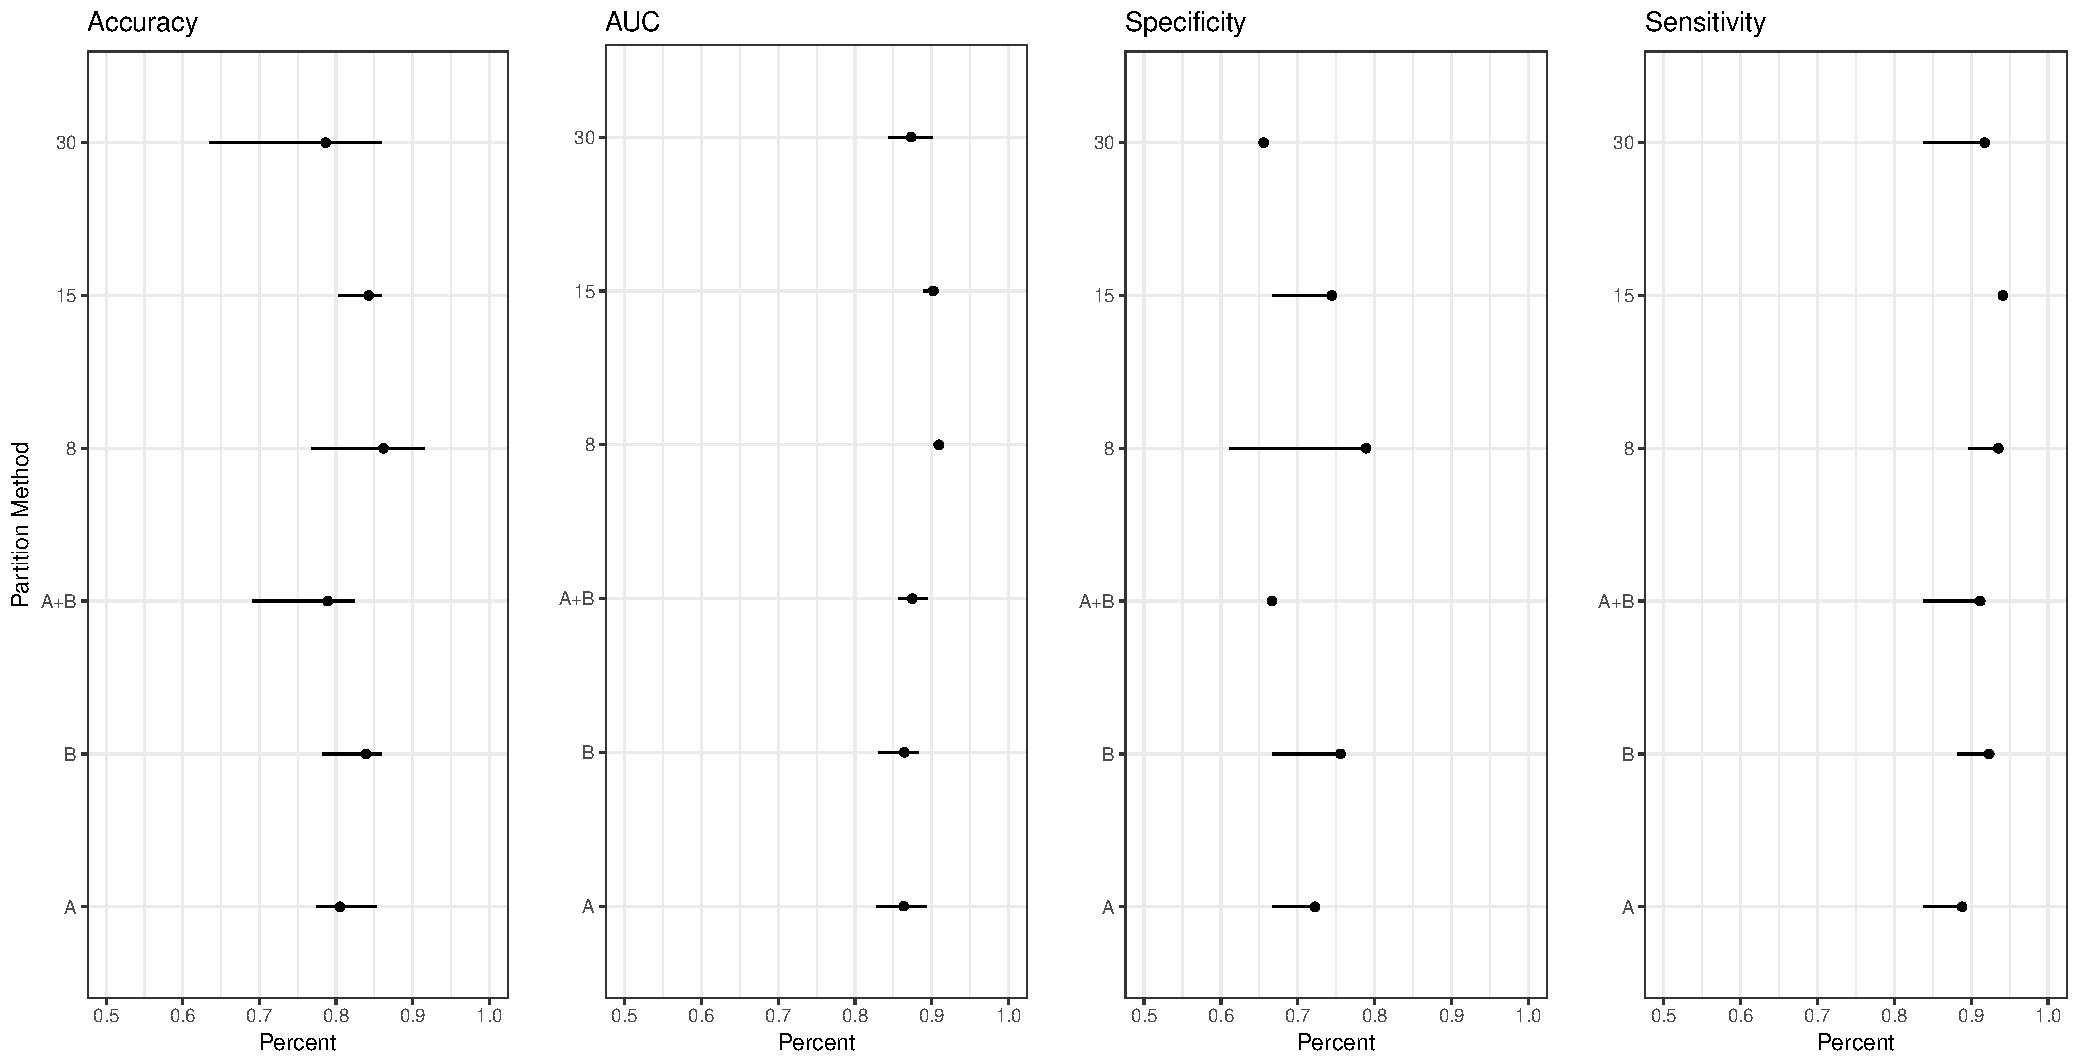
\includegraphics[width = \textwidth, keepaspectratio]{./figs/eeg-partition-diagnostic.pdf}
  % \end{picture}
  \end{center}
  \caption{Classification diagnostic values for each classifier using
   features LFP channel 1.}
  \label{fig:eeg-diagnostic} 
\end{figure}

The mean and 95\% confidence intervals for the 
performance measures for each classifier using features
computed on channel are shown in Figure \ref{fig:eeg-diagnostic}.
All methods classified non-response trials well but the two better performing
 models --- model 8  and model $B$ --- 
had relatively high accuracy in classifying seizure responses: 76\% for model $B$ and 79\% for model 8. 

% Table created by stargazer v.5.2 by Marek Hlavac, Harvard Unaiversity. E-mail: hlavac at fas.harvard.edu
% Date and time: Tue, Jul 11, 2017 - 02:07:16 AM
\begin{table}[!htbp] \centering 
\begin{tabular}{@{\extracolsep{-5pt}} ccccccccccccc} 
\\[-1.8ex]\hline 
\hline \\[-1.8ex] 
 & CH1 & (sd1) & CH2 & (sd2) & CH3 & (sd3) & CH4 & (sd4) & CH5 & (sd5) & CH6 & (sd6) \\ 
\hline \\[-1.8ex] 
A & 0.82 & (0.04) & 0.77 & (0.04) & 0.69 & (0.02) & 0.71 & (0.04) & 0.57 & (0.04) & 0.63 & (0.03) \\ 
B & 0.83 & (0.03) & 0.77 & (0.04) & 0.71 & (0.03) & 0.71 & (0.03) & 0.61 & (0.05) & 0.65 & (0.06) \\ 
A+B & 0.81 & (0.03) & 0.73 & (0.03) & 0.70 & (0.04) & 0.72 & (0.03) & 0.57 & (0.09) & 0.63 & (0.07) \\ 
8 & 0.83 & (0.05) & 0.82 & (0.04) & 0.74 & (0.04) & 0.72 & (0.02) & 0.75 & (0.05) & 0.74 & (0.06) \\ 
15 & 0.82 & (0.05) & 0.84 & (0.04) & 0.73 & (0.04) & 0.73 & (0.02) & 0.77 & (0.05) & 0.78 & (0.06) \\ 
30 & 0.79 & (0.07) & 0.77 & (0.05) & 0.76 & (0.04) & 0.76 & (0.03) & 0.73 & (0.08) & 0.75 & (0.04) \\ 
\hline \\[-1.8ex] 
\end{tabular} 
  \caption{Mean and s.d. of balanced accuracy for all models.} 
  \label{tab:all-accuracy} 
\end{table} 
% Table created by stargazer v.5.2 by Marek Hlavac, Harvard University. E-mail: hlavac at fas.harvard.edu
% Date and time: Tue, Jul 11, 2017 - 02:06:02 AM
\begin{table}[!htbp] \centering 
\begin{tabular}{@{\extracolsep{-5pt}} ccccccccccccc} 
\\[-1.8ex]\hline 
\hline \\[-1.8ex] 
 & CH1 & (sd1) & CH2 & (sd2) & CH3 & (sd3) & CH4 & (sd4) & CH5 & (sd5) & CH6 & (sd6) \\ 
\hline \\[-1.8ex] 
A & 0.73 & (0.06) & 0.60 & (0.08) & 0.46 & (0.04) & 0.52 & (0.05) & 0.26 & (0.07) & 0.33 & (0.05) \\ 
B & 0.76 & (0.07) & 0.59 & (0.07) & 0.51 & (0.06) & 0.53 & (0.05) & 0.37 & (0.09) & 0.38 & (0.11) \\ 
A+B & 0.69 & (0.07) & 0.51 & (0.06) & 0.49 & (0.08) & 0.53 & (0.05) & 0.23 & (0.17) & 0.32 & (0.12) \\ 
8 & 0.77 & (0.11) & 0.70 & (0.07) & 0.59 & (0.07) & 0.54 & (0.04) & 0.62 & (0.11) & 0.57 & (0.11) \\ 
15 & 0.71 & (0.09) & 0.73 & (0.08) & 0.57 & (0.06) & 0.56 & (0.00) & 0.68 & (0.12) & 0.62 & (0.12) \\ 
30 & 0.64 & (0.14) & 0.60 & (0.09) & 0.60& (0.08) & 0.61 & (0.06) & 0.59 & (0.15) & 0.58 & (0.09) \\ 
\hline \\[-1.8ex] 
\end{tabular} 
  \caption{Mean and s.d. of specificity for all models.} 
  \label{tab:all-specificity} 
\end{table}


The balanced accuracy of all models for each channel is
reported in Table \ref{tab:all-accuracy}. All partition
schemes resulted in fairly high rates of accuracy for channels 1 and 2. The models with a higher number of 
partitions performed significantly better on the 
iEEG channels 3-6. Accurate classification of seizures tailed off sharply for all iEEG channels as seen in Table \ref{tab:all-specificity}. In particular, specificity was greater than 70\% for only 
a few models, all of which used channels 1 or 2. The ROC and smoothed ROC curves in Figure \ref{fig:eegroc}
for are similar for both the model $A + B$ and model $8$. 


\begin{figure}[!htbp]
  \begin{center}
  % \begin{picture}(60,60)
  % ./figs/coeff-interp-simple-functions1.pdf
  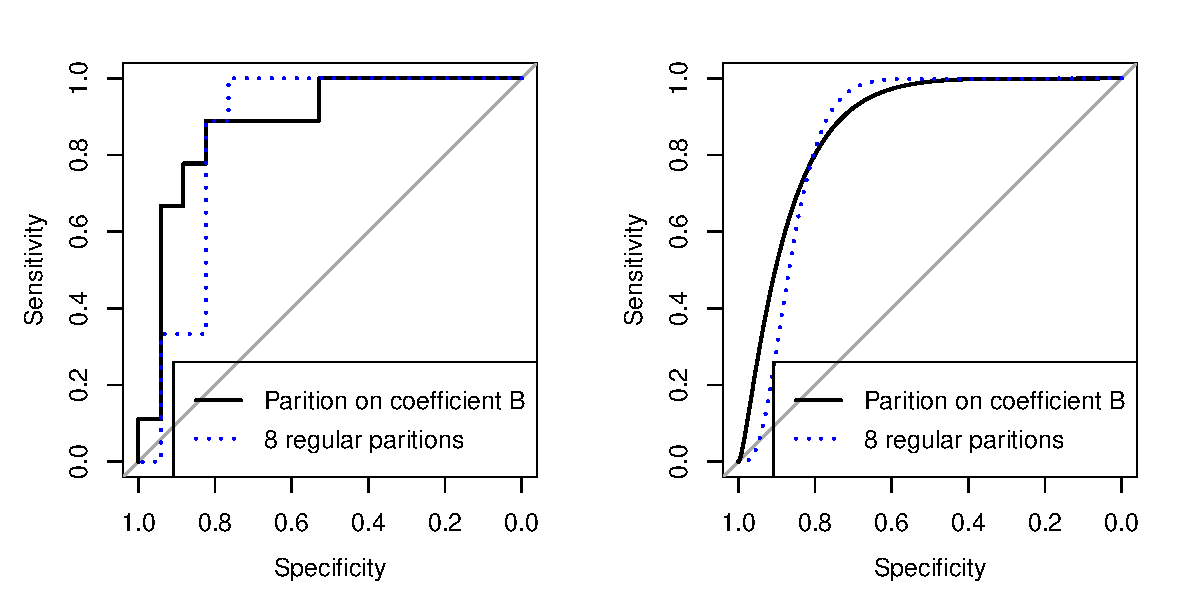
\includegraphics[width = \textwidth, keepaspectratio]{./figs/eegroc-comb.pdf}
  % \end{picture}
  \end{center}
  \caption{Best ROC curves for classifiers $B$ and $8$.}
\end{figure}
\label{fig:eegroc} 




\section{Feature Importance}

% \begin{table}[!htbp]
% \begin{center}
%   \begin{tabular}{ | c | c |  c| c | c | c |c| } 
%   \hline 
% Channel       &     1&    2 &    3 &     4 &     5 &    6  \\ \hline
% Partition Type    &       &      &     &     &  &  \\ \hhline{|=|=|=|=|=|=|=|}
% A    & 0.81 & 0.78 & 0.69 & 0.72  & 0.57  & 0.63  \\ \hline
% B    & 0.84 & 0.77 & 0.72 & 0.70  & 0.57  & 0.65  \\ \hline
% A+B  & 0.81 & 0.74 & 0.73 & 0.72  & 0.55  & 0.60  \\ \hline
% 8    & 0.86 & 0.84 & 0.73 & 0.72  & 0.74  & 0.75  \\ \hline
% 15   & 0.85 & 0.81 & 0.74 & 0.73  & 0.75  & 0.75  \\ \hline
% 30   & 0.79 & 0.75 & 0.76 & 0.77  & 0.72  & 0.77  \\ \hline
%       \end{tabular}  
% \caption{Balanced classification accuracy for each partition method 
%          and each channel.}
% \label{tab:error-allch}
% \end{center}
% \end{table}

% Table created by stargazer v.5.2 by Marek Hlavac, Harvard University. E-mail: hlavac at fas.harvard.edu
% Date and time: Sun, Jun 25, 2017 - 10:27:00 PM
 

The classification results show that seizures could with 
a relatively high degree of accuracy for some model 
and channel combinations. Apart from the baseline 
model, each of these models used features calculated 
on individual channels. This allows us to look at 
the combination of feature and channel 
associated with accurate predictions. Here 
we compare the variable importance of the more successful 
models to the difference in feature distributions 
between trials with a seizure and non-seizure response.
Random forests build multiple decision trees that divide up the feature space in complex ways and the final classification is
tallied from the votes of individual trees. This means there 
may be now clear relation between feature distribution and 
random forest variable importance. Nevertheless, we find that 
features associated with the best predictors were associated
with clear differences in distributions between trial classes.

%  in particular 
% the features trained on predictors trained on the LFP channels 1 and 2. 

\begin{figure}[h]
  \begin{subfigure}[b]{0.45\textwidth}
      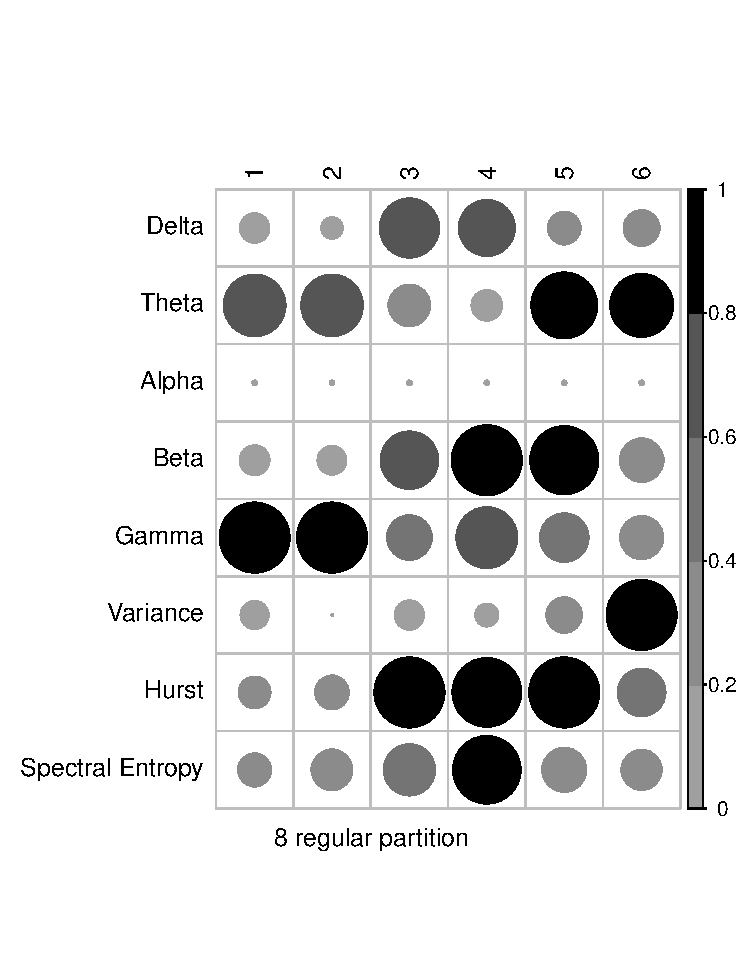
\includegraphics[width = \linewidth, keepaspectratio]{./figs/eeg-vec-corrplot.pdf}% \end{picture}
    % \caption{Functions without added noise.}
    % \label{fig:corrplot}
  \end{subfigure} 
  \hfill
  \begin{subfigure}[b]{0.45\textwidth}
    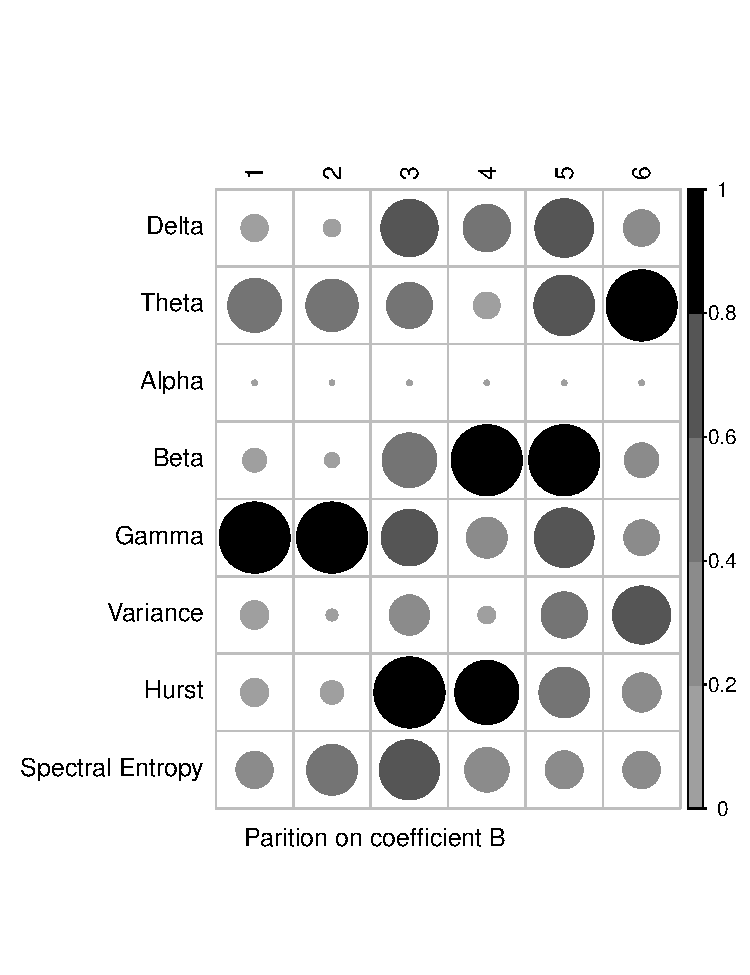
\includegraphics[width = \linewidth, keepaspectratio]{./figs/eeg-AB-corrplot.pdf}% \end{picture}
  % 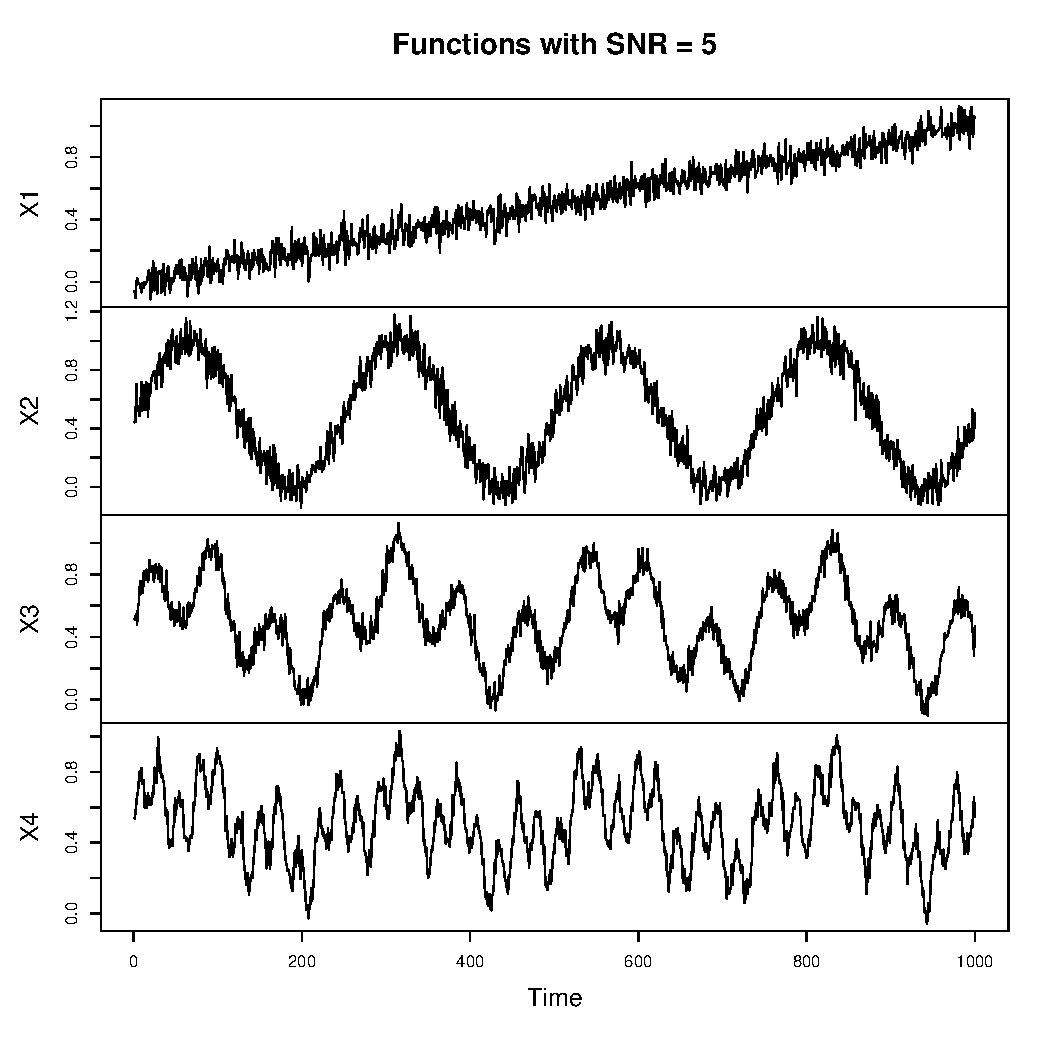
\includegraphics[width = 0.9\linewidth, height = 3in]{./figs/coeff-interp-simple-functions1.pdf}
    % \caption{Functions without added noise.}
      \end{subfigure}
  \caption{Normalized variable importance for
     each partition method and channel.}
    \label{fig:corrplot}
\end{figure}

In Figure \ref{fig:corrplot} we show the variable 
importance for the two best performing models $B$ and the 
model $8$. We have normalized variable importance to a $[0,1]$ interval for each model and
channel so the figure shows the relative importance of the variable for each model. There is a common pattern in the variable importance across the two models. Gamma and theta bands have the highest importance for the best performing models, those trained on the LFP channels 1 and 2. Both partition methods also show increased importance for beta on channels 4 and 5 and increase the importance of the Hurst coefficient for channels 3 and 4. However, no model 
was able to accurately predict seizures using these channels 
in isolation. The maximum specificty among all models trained 
on these channels was 68\% and for the two models depicted 
in \ref{fig:corrplot} this number was 59\%. 

\begin{figure}[!htbp]
  \begin{subfigure}[b]{ \textwidth}
  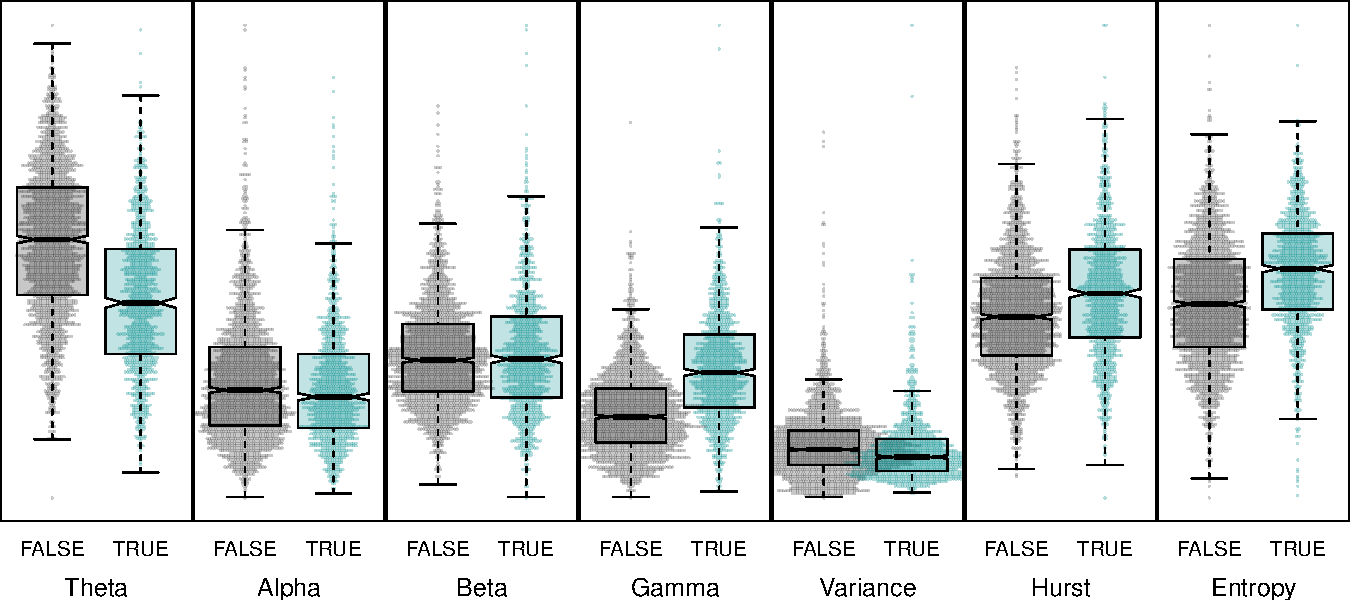
\includegraphics[width = \textwidth, keepaspectratio]{./figs/eeg-boxplot1.pdf}
    % \label{fig:corrplot}
  \end{subfigure} 
  \hfill
  \begin{subfigure}[b]{\textwidth}
  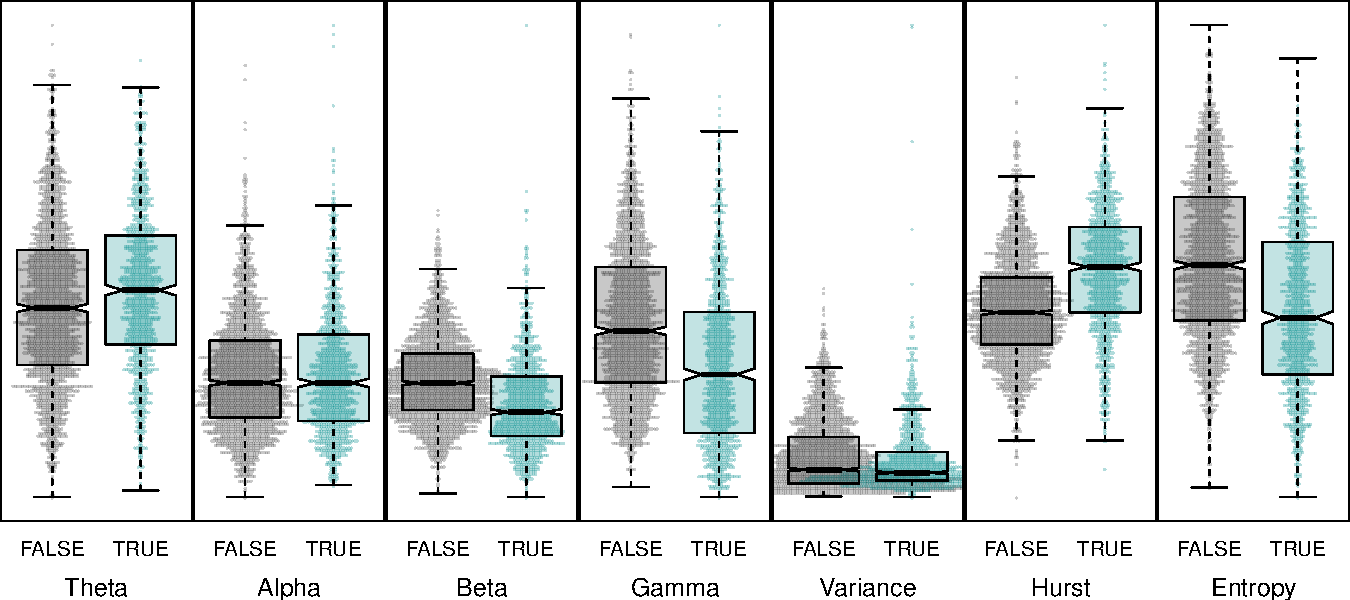
\includegraphics[width = \textwidth, keepaspectratio]{./figs/eeg-boxplotch3.pdf}
  % 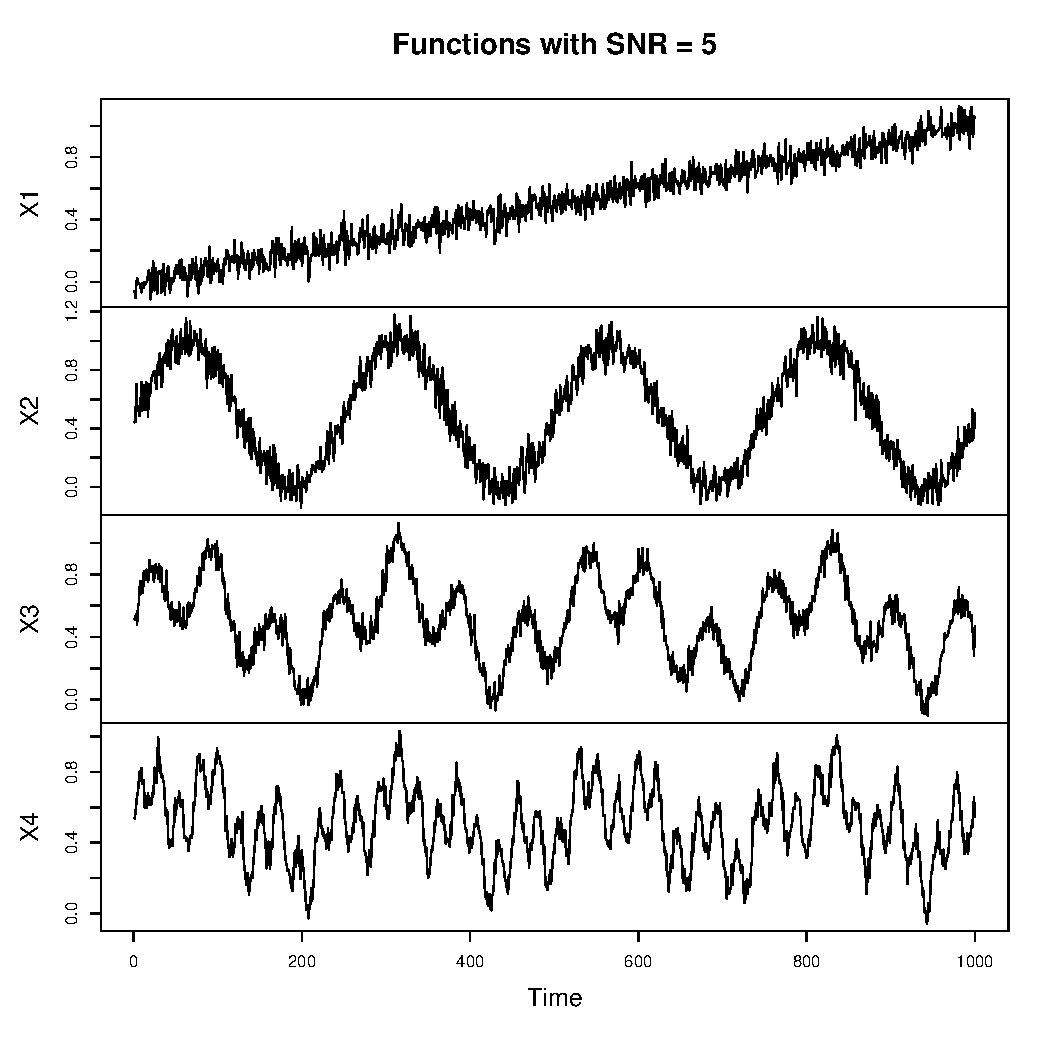
\includegraphics[width = 0.9\linewidth, height = 3in]{./figs/coeff-interp-simple-functions1.pdf}
    % \caption{Functions without added noise.}
      \end{subfigure}
  \caption{Feature distribution for channels 1 and 3.}
  \label{fig:boxplot}
\end{figure}

% \begin{figure}[!htbp]
%   \begin{center}
%   % \begin{picture}(60,60)
%   % ./figs/coeff-interp-simple-functions1.pdf
%   % \end{picture}
%   \end{center}
%   \label{fig:eegroc} 
%   \caption{Feature distribution for channel 1.}
% \end{figure}

% \begin{figure}[!htbp]
%   \begin{center}
%   % \begin{picture}(60,60)
%   % ./figs/coeff-interp-simple-functions1.pdf
%   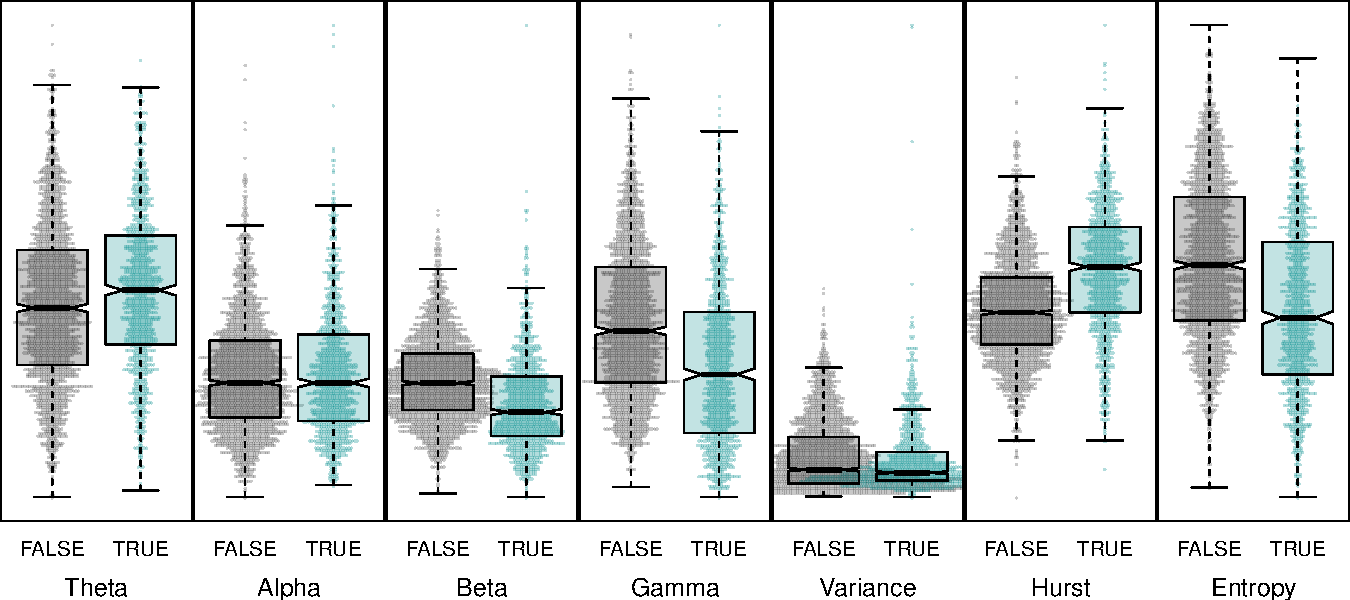
\includegraphics[width = \textwidth, keepaspectratio]{./figs/eeg-boxplotch3.pdf}
%   % \end{picture}
%   \end{center}
%   \label{fig:eegroc} 
%   \caption{Feature distribution for channel 1.}
% \end{figure}

Variable importance as measured by the random forest classifiers 
was also reflected in distributional differences in the features. 
The box plots in figure \ref{fig:boxplot} show the distribution 
and features for channels 1 and 3.  For channel 1, the relative 
power of gamma is higher and theta lower for trials with 
seizure responses. The median of theta and gamma fall outside the inter-quartile range and a similar distribution was similar for channel two.  For channel three, the relative power of theta
and gamma are reversed with gamma lower and theta higher. 
On the other hand, the distribution of beta for channels 1 and 2 
were similar while beta was significantly lower for channels 3 and 4. Table \ref{tab:pvals}
shows the p-value determined by the unpaired 
Wilcox rank-sum test, a nonparametric test of
the difference between two distributions. While a large number of data points guarantees that even small differences will be statistically significant, the table does highlight the non-significant values. 


% Table created by stargazer v.5.2 by Marek Hlavac, Harvard University. E-mail: hlavac at fas.harvard.edu
% Date and time: Mon, Jun 26, 2017 - 08:05:44 PM

\begin{table}[!ht] \centering 
\begin{tabular}{@{\extracolsep{5pt}} ccccccc} 
\\[-1.8ex]\hline 
\hline \\[-1.8ex] 
 Channel & 1 &  2 &  3 &  4 & 5 &  6 \\ 
\hline \\[-1.8ex] 
Delta & $< .0001$ & $< .0001$ & $< .0001$ & $< .0001$ & $< .0001$ & $< .0001$ \\ 
Theta & $< .0001$ & $< .0001$ & $< .0001$ & $< .0001$ & $< .0001$ & $< .0001$ \\ 
Alpha & $0.022$ & $0.699$ & $0.897$ & $0.891$ & $0.008$ & $0.302$ \\ 
Beta & $0.826$ & $0.226$ & $< .0001$ & $< .0001$ & $< .0001$ & $< .0001$ \\ 
Gamma & $< .0001$ & $< .0001$ & $< .0001$ & $< .0001$ & $< .0001$ & $< .0001$ \\ 
Variance & $< .0001$ & $< .0001$ & $0.687$ & $0.005$ & $< .0001$ & $< .0001$ \\ 
Hurst & $< .0001$ & $< .0001$ & $< .0001$ & $< .0001$ & $< .0001$ & $< .0001$ \\ 
Spectral Entropy & $< .0001$ & $< .0001$ & $< .0001$ & $< .0001$ & $0.0003$ & $< .0001$ \\ 
\hline \\[-1.8ex] 
\end{tabular} 
  \caption{P-values fo Wilcox rank sum test 
   for difference of distribution} 
  \label{tab:pvals} 
\end{table} 

\section{Discussion} 

While we were able to predict a seizure result 
with relatively high accuracy using several 
classification methods, there are some 
limitations to the study. There were 4 mice 
used in the experiments but the 
trials resulting in seizures came from a single mouse.
Data from other mice would be 
required to know whether the features associated 
with seizures held more generally. In addition, 
most of the seizures 
came from stimuli applied within two trials. 
Several of the seizures responses, then, 
occurred after a previous seizure. 
Therefore, features found predictive of a seizure may  
be conflated with features that are a result of a seizure. 
% As mentioned in the limitations section, the seizure responses 
% came in all cases from a single mouse and most of those 
% seizures came in trial periods during which there was more than one 
% seizure. Whether the predictive model generalizes to other cases
% and whether the differences in features that were predictive of 
% a seizure are similar for other subjects remains open. 
Due to the small number of trials, we did not 
have a hold-out data set. The lab from which produced this 
set of data is collecting additional data.  
Testing the predicitive models described here against 
new data would better indicate whether the predictive power 
generalize well.

% Although feature importance seemed robust to changes 
% in the partitions comparing feature performance across other 
% predictive models 
The segmentation model based on the complexity coefficients performed as the models with regular partitions for some channels.  However, the regular partition models tended to perform more consistently across channels. The models built using channels 
the iEEG electrodes, channels 3-6, the models using features 
partitioned at regular intervals performed better than the 
models partitioned on change points in
$\varepsilon-$complexity. The algorithm used to detect
changes points in the complexity coefficients was sensitive to 
the density at which the features were computed. For example, 
computing the features, including the complexity coefficients 
on an overlapping set of windows would increase the density at 
which features were calculated. A finer resolution may 
improve the detection of change points the complexity coefficients. 
On average, the uniform partitions created divided the 
trials into more segments. It may also simply be that a somewhat 
finer segmentation than that given by the complexity coefficients
is what improved the consistency of the models with uniform 
partitions. 
Tests of this segmentation model on simulated data sets or a wider range of time series would be needed to assess the performance of the model in more general contexts.  


% One of our assumptions was that arbitrary partitioning would average over changes variations in the features that corresponded to transient states. 
% But whether the complexity coefficients capture significant
% changes in the underlying dynamics that are useful for classification might depend on both feature selection and the classification task. 

% As mentioned above, with only a small set of observations, 
% improved classification on one or two instances
% would affect the performance of the classifier.
% Whether the model used here --
% partitions based on complexity coefficients -- would be successful in other contexts remains to be seen. 






